\chapter{Windows development}

In the previous chapters, we delved into the world of eBPF and explored its versatile capabilities within the Linux ecosystem.
But eBPF is now a cross-platform technology: we are going to continue our journey beyond the confines of Linux to explain the possibilities of eBPF development on the Windows operating system. 
This chapter serves as a guide for developers and enthusiasts that want to utilize the power of eBPF for Windows-centric applications.

While eBPF is natively integrated into the Linux kernel, recent advancements have extended its reach to the Windows platform, making it accessible to a broader audience. 
This development opens up new horizons for network monitoring, security and performance analysis within Windows environments.

Since May 2021, Microsoft has been working on bringing eBPF to Windows. 
In fact, in recent times there have been significant developments in the integration of eBPF on the this platform. 
As of the time of writing this thesis in September 2023, eBPF for Windows is in a state of rapid evolution and expansion. 
In this chapter we’ll be looking at setting up a Windows-eBPF build environment, followed by developing, running and debugging eBPF programs on Windows, providing insights into its current status and potential future directions. 

Unlike what we saw for linux, to date there is only one way to work with eBPF on Windows: it involves using the \textit{ebpf-for-windows} open-source GitHub project by Microsoft \cite{eBPFWinGitHubRepo}.
This repository is full of documents that describe how to to get started and use eBPF on Windows.
We will make several references to these documents to avoid making the reading too heavy, but we will highlight the crucial passages.
To start working with ebpf on Windows, in fact, the experience is not as user-friendly as it was on Linux where it was enough to clone a repository.
This statement is not intended to discourage anyone, but it will immediately be clear that not so much the coding part as the setup of an environment will be very long and complex.

Moreover, we are going to present another project, called \textit{windows-ebpf-starter}, that was created to make the experience of eBPF programming within the Windows ecosystem easier \cite{WineBPFStarterRepo}: the result is that this project is for Windows what libbpf-bootstrap is for Linux.
However, at the time of writing, the parallelism is not true in every aspect: we are going to present later some issues that we came across while developing eBPF applications.

\section{Creation of the work environment}

In the previous chapter mentioned the fact that we needed a Linux environment in which we could develop various programs: to do so, we used VirtualBox.
Now we have to create another environment, this time for Windows, as we will study the state of the art of eBPF on this latest operating system. 

Remembering that the computer on which the process was carried out has Windows 11 as its operating system, for this purpose we used the \textit{Hyper-V Console Manager}, a native Windows feature, to create a separate Windows 11 virtual machine.
\textit{Hyper-V} is a type 1 (or bare-metal) virtualization software, also known as a \textit{Virtual Machine Monitor} (\textit{VMM}), which runs directly on the physical hardware without the need for an underlying host operating system. 
The illustrative representation of the architecture just described is depicted in Figure \ref{fig:type_1_hypervisor}.
As the core software responsible for managing virtual machines and allocating hardware resources to each VM, Hyper-V ensures better security and resource utilization by isolating each VM from others and the host OS. 
With direct access to the physical hardware, it efficiently allocates resources, resulting in improved performance, isolation and scalability compared to type 2 hypervisors like VirtualBox.

\begin{figure}[h]
	\centering
	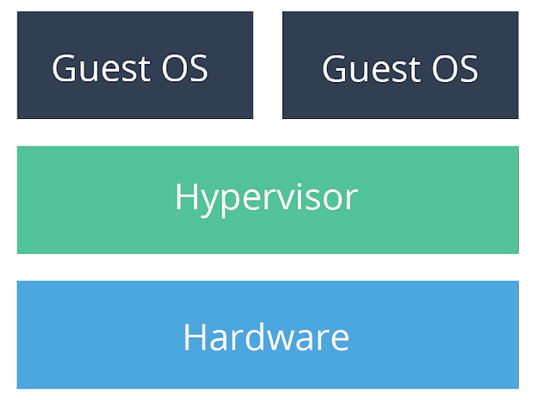
\includegraphics[width=0.7\linewidth]{images/Technologies/type_1_hypervisor.png}
	\caption{Type 1 (or bare metal) hypervisor architecture \cite{HypervisorsArchitectures}.}
	\label{fig:type_1_hypervisor}
\end{figure}

The greatest benefits of hypervisors are their robustness and scalability, enabling the efficient virtualization of large-scale applications and services.
However, the choice of creating a virtual machine using the Hyper-V Console Manager was dictated by two other reasons:

\begin{itemize}
	\item 
		The setup instructions described on the ebpf-for-windows GitHub repository tell the user to install a Windows virtual machine;
	\item 
		The so created isolated Windows 11 development environment provided a controlled space for testing and optimizing eBPF programs on the Windows platform.
		In fact, if anything goes wrong in this environment, we can just delete the virtual machine and create a new one, while if something bad happens on our host machine, we could break our computer.
\end{itemize}

So, to install eBPF on Windows the first thing that we have to do is to install our virtual machine.
To do so, we have to follow the instructions reported in the \textit{vm-setup.md} document \cite{WinVMSetupDoc}.
Besides the fact that that the virtual machine was configured with adequate resources to support development tasks effectively, the only thing worth noting is that during the quick creation of the virtual machine the option of ``Windows 11 dev environment'' is the only one that can be selected since our host computer has Windows 11 as operative system (the tutorial tells to choose the ``Windows 10 dev environment'' probably because at the time of writing of this document version 10 of Windows was the highest available, but Windows 11 works as well).  

After the ``one-time setup'' procedure is done, we have to decide how we are going to debug our virtual machine.
After a careful analysis of the requirements needed to install eBPF we decided to configure a kernel debugging connection over IP address.
In fact, since the eBPF for Windows binaries are not yet signed by Microsoft, they will only work on a machine with a kernel debugger attached and running or test signing is enabled.
Between the two, we decided to took the first route because it seemed easier.
To do so there are a few articles on the Microsoft Learn website, under the documentation section, that we have (once again) to follow by heart.
The two things that are worthy of note with this approach are the following:

\begin{itemize}
	\item 
		On our host computer we have to install a set of debugging tools for Windows.
		There are a few available \cite{DbgToolsWin}, but we decided to stick with the classic \textit{WinDbg}, a debugger that can be used to analyze crash dumps, debug live user-mode and kernel-mode code, and examine CPU registers and memory \cite{InstallWinDbg}.
		After following the installation path of this tool, we will find it under \lstinline[style=commandline, language=bash]|C:\Program Files (x86)\Windows Kits\10\Debuggers\x64|;
	\item 
		Since it is very likely that sometimes we will shut down our virtual machine, every time that we are going to turn it on we have to start the kernel debugger attached to it (we will present later how to do it).
		This is quite inconvenient due to the fact that it requires a bit of time every time.  
\end{itemize}

At this point we have all the components that we will need on our host computer.
Now we have to install a series of applications on the virtual machine: under the \textit{Prerequisites} of \textit{Building eBPF for Windows} in the \textit{GettingStarted.md} document there is a list of things to install in order to build the repository project \cite{GetStartDoc}.
Moreover, to make WinDbg work and debug the virtual machine over IP, we have to install \textit{KDNET}, a debugging feature in Windows that allows remote kernel debugging over a network connection.

Once we have installed all the required tools, we are ready to start debugging our virtual machine.
With KDNET we have to set up the target machine (the one we want to debug) and the host machine (the one we will use for debugging) to communicate and then we can start the debugging session: an article on the Microsoft Learn websites tells us what to do \cite{SetUpNetDebug}.
However, even after we have followed all the listed steps the first time, whenever we want to turn on our virtual machine to work with eBPF, we have to redo some of these steps.
In particular, we have to:

\begin{itemize}
	\item 
		Open a \textit{Command prompt} with administrator privileges on both the machines;
	\item 
		Check the host IP address with the command \lstinline[style=commandline, language=bash]|ipconfig| because if we let the \textit{Dynamic Host Configuration Protocol} (\textit{DHCP}, a network management protocol used on IP networks for automatically assigning IP addresses and other communication parameters to devices connected to the network using a client–server architecture) to assign automatically an IP address to our computer the address may vary;
	\item 
		On the virtual machine, in the \lstinline[style=commandline, language=bash]|C:\KDNET| folder (that we should have created if we followed the last mentioned article) we have to run \lstinline[style=commandline, language=bash]|C:kdnet <YourIPAddress> <YourDebugPort>|, where the debug port must be within the range 50000-50039.
		This command will give us another command that we have to copy and run on the host machine.
		It will look like this: \lstinline[style=commandline, language=bash]|windbg -k net:port=<YourDebugPort>,key=<YourKey>|, where the key consists of four alphanumeric strings separated by three dots;
	\item 
		On our host machine we have to:
		\begin{itemize}
			\item 
				Go to the folder where wh have installed WinDbg, which is \lstinline[style=commandline, language=bash]|C:\Program Files (x86)\Windows Kits\10\Debuggers\x64|;
			\item 
				Run the command that we have copied from the virtual machine.
		\end{itemize}
		After we have run the command, WinDbg will start on our host machine.
		However, for now, it says ``Debuggee not connected''.
		We have to do a couple more steps to make it work;
	\item 
		Disable \textit{Enhanced session} on the virtual machine using the \textit{View} pull down menu in the VM;
	\item 
		Restart the virtual machine with the command \lstinline[style=commandline, language=bash]|shutdown -r -t|.	
		If after we restart the virtual machine one time the ``Debuggee not connected'' string did not change, we have to restart it a second time.
		If we do so, we should be able to see ``Debugger is running...''.
\end{itemize}

After everything is done we now have started our virtual machine with a kernel debugger attached.
\todo{FIGURE BEFORE AND AFTER THE TURN ON OF THE DEBUGGER}

At this point, remember to do the last point on the \textit{vm-setup.md} document which is \textit{Enable Driver Verifier on eBPF drivers}.

The last step that we have to make is to install ebpf-for-windows.
To do so, we have to follow the instructions given by the \textit{InstallEbpf.md} document \cite{InseBPFDoc}.
The easiest way to install eBPF into a test virtual machine is to stick to the so called \textit{Method 1}.
For this thesis we worked with the \textit{v0.9.0} version, but at the time of writing versions \textit{v0.10.0} and \textit{v0.11.0} were released.
We can understand how fast this technology is evolving on Windows.

Once we have done with all the set up part, we can now start developing some examples using the ebpf-for-windows project.
We must point out that from now on we will assume that we are working on a virtual machine that has been turned on with a kernel debugger attached, as we explained previously.

\section{ebpf for Windows}

% https://microsoft.github.io/ebpf-for-windows/ -> MANUAL PAGE

% https://github.com/Microsoft/ebpf-for-windows/ 

To develop eBPF applications on Linux we used two projects that made this task relatively simple once we understood the logic behind eBPF.
Unfortunately, with ebpf-for-windows this doesn't happen.
However, the repository provides several documents in which it explains how to develop simple initial programs and how to debug them.

But before doing so, we have to build our project: to do so, we have to follow the ``How to clone and build the project using Visual Studio'' section in the \textit{GettingStarted.md} document which consists of some operations besides cloning the repository.

\cite{TutDoc}

\cite{DebugDoc}

\section{windows ebpf starter}

% https://blog.subcom.tech/ebpf-programming-on-windows/

% https://github.com/SubconsciousCompute/windows-ebpf-starter